\documentclass{estacio}

\usepackage{listings} % Pacote para inclusão de códigos

% Configuração do ambiente para códigos Python
\lstnewenvironment{pythoncode}[1][]{
    \lstset{
        language=Python,
        basicstyle=\scriptsize\ttfamily, % Altere para \scriptsize ou \small
        keywordstyle=\color{blue!70!black}\bfseries,
        stringstyle=\color{orange!70!black},
        commentstyle=\color{green!70!black}\itshape,
        morecomment=[l][\color{magenta}]{\#},
        numbers=left,
        numberstyle=\tiny\color{gray}, % Tamanho das linhas numeradas
        stepnumber=1,
        numbersep=5pt,
        tabsize=4,
        showspaces=false,
        showstringspaces=false,
        breaklines=true,
        frame=tb,
        framexleftmargin=5mm,
        aboveskip=3mm,
        belowskip=3mm,
        captionpos=b,
        #1
    }
}{}

\begin{document}
\maketitle

\section{Resumo Executivo}
Este relatório aborda a simulação de inicialização de LEDs em microcontroladores Arduino ou ESP32 por meio da plataforma online Tinkercad. Apresenta-se uma visão geral dos passos para realizar a simulação, suas aplicações práticas e a importância dessa prática para o aprendizado e desenvolvimento de habilidades em eletrônica e programação embarcada.

\section{Introdução}
A simulação de inicialização de LEDs é uma etapa essencial no aprendizado de programação embarcada e controle de hardware. Esta prática permite aos usuários entenderem os fundamentos da programação de microcontroladores e como controlar dispositivos de saída, como os LEDs, de forma eficiente.

\section{Plataforma Escolhida}
O Tinkercad foi selecionado como a plataforma para realizar a simulação. O Tinkercad oferece uma interface amigável e poderosas ferramentas de design para criar e testar circuitos eletrônicos e programação de microcontroladores em um ambiente virtual.

\section{Passos para Simulação}
\begin{enumerate}
    \item \textbf{Acesso à Plataforma:} Acesse o site do Tinkercad e faça login em uma conta gratuita, se necessário.
    \item \textbf{Configuração do Circuito:} Utilize o editor de circuitos para adicionar um microcontrolador Arduino ou ESP32 à área de trabalho.
    \item \textbf{Adição de LEDs:} Adicione LEDs à placa do microcontrolador e conecte-os aos pinos de saída digital.
    \item \textbf{Escrita do Código:} Escreva o código em linguagem de programação Arduino para simular a inicialização dos LEDs, como fazer os LEDs piscarem em sequência.
    \item \textbf{Upload e Simulação:} Faça o upload do código para o microcontrolador na plataforma Tinkercad e inicie a simulação para observar o comportamento dos LEDs conforme o código programado.
\end{enumerate}

\section{Aplicação Prática}
A simulação de inicialização de LEDs em Arduino ou ESP32 tem diversas aplicações práticas, incluindo:
\begin{itemize}
    \item \textbf{Aprendizado de Programação:} Permite que iniciantes pratiquem programação de microcontroladores de forma segura e interativa.
    \item \textbf{Prototipagem Rápida:} Possibilita que desenvolvedores testem e depurem seus códigos antes de implementá-los em hardware real, economizando tempo e recursos.
    \item \textbf{Educação em Engenharia:} Professores podem usar essa ferramenta para ensinar conceitos de eletrônica e programação de forma envolvente e prática.
\end{itemize}

\section{Conclusão}
A simulação de inicialização de LEDs em Arduino ou ESP32 por meio do Tinkercad é uma prática valiosa para o aprendizado e desenvolvimento de habilidades em eletrônica e programação embarcada. Ao explorar essa ferramenta, os usuários podem adquirir conhecimentos essenciais para projetar e desenvolver sistemas embarcados com eficiência e precisão.

\section{Anexo}
\begin{figure}[h]
    \centering
    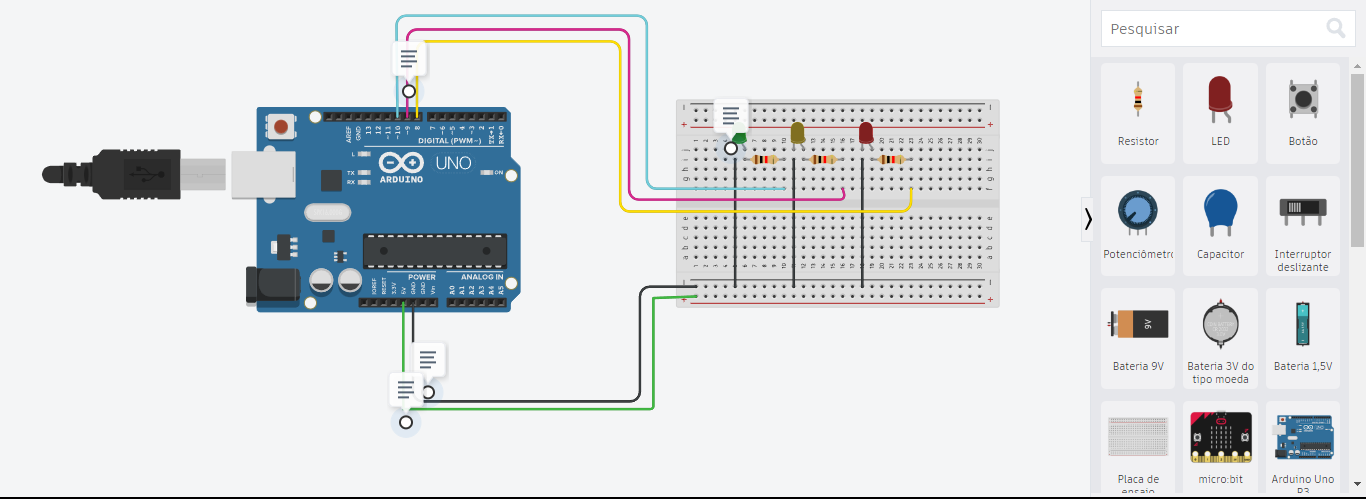
\includegraphics[width=0.5\textwidth]{assets/arduino.png}
    \caption{Simulação de inicialização de LEDs em Arduino no Tinkercad.}
    \label{fig:simulacao_tinkercad}
\end{figure}

\end{document}